\section{Method}
\label{sec:method}

% Role: overview.
\paragraph{Overview.}
\method allocates W4A8 and FP16 at layer granularity without updating pretrained parameters. The method has four stages, illustrated in Fig.~\ref{fig:pipeline}: (i) an isolated intervention protocol measures the effect of quantizing one layer; (ii) dual-similarity scores describe representation geometry and distribution shift; (iii) an action-weighted constrained selector proposes diverse precision masks; and (iv) paired functional adjudication chooses complete configurations before a closed-loop development set freezes the metric ratio. This organization separates inexpensive layer attribution from the cross-layer behavior that ultimately determines control quality.

\begin{figure*}[t]
    \centering
    \IfFileExists{figures/gdsq_pipeline.png}{%
        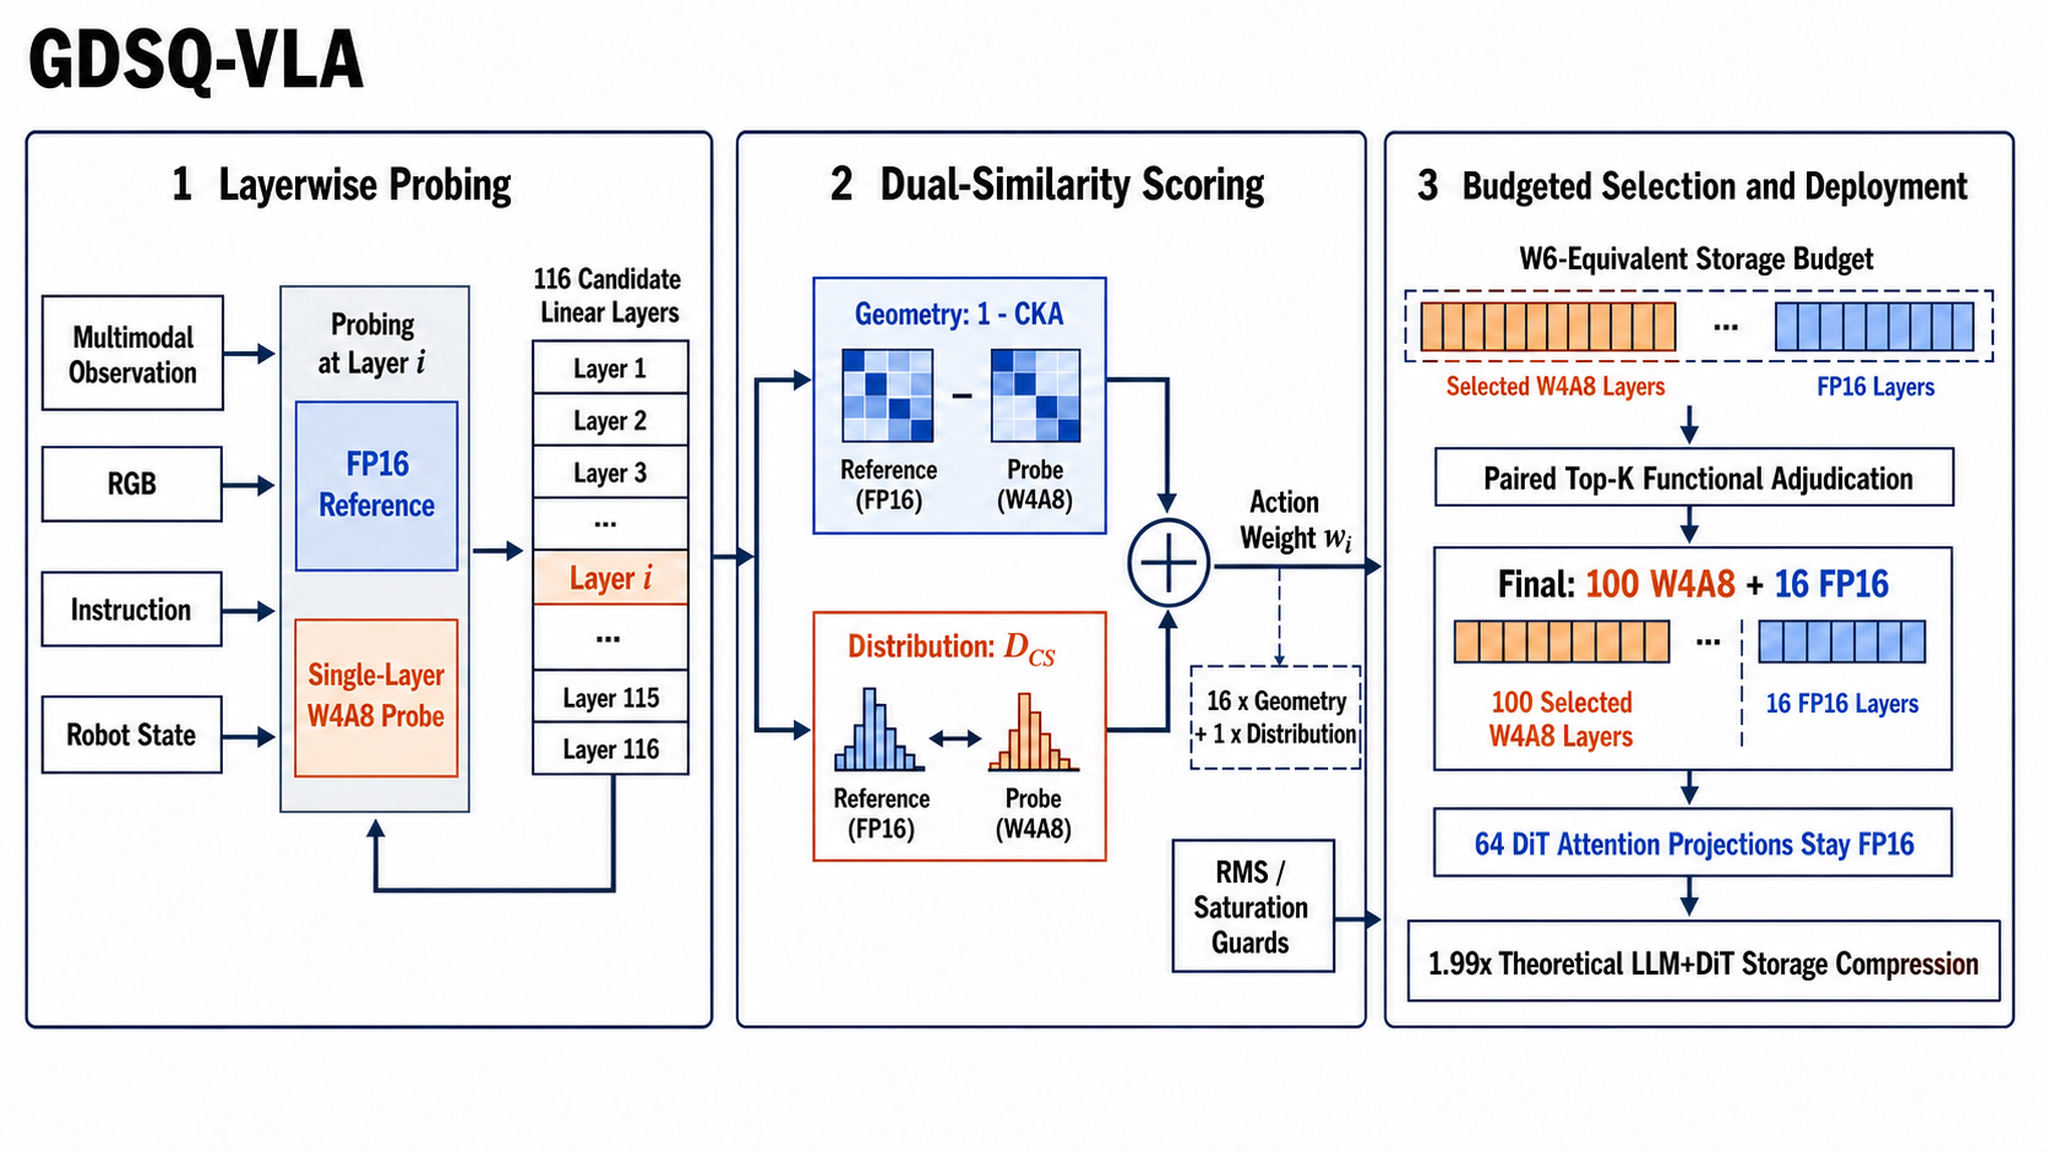
\includegraphics[width=\textwidth]{figures/gdsq_pipeline.png}%
    }{%
        \setlength{\fboxsep}{7pt}%
        \fbox{%
        \begin{minipage}{0.96\textwidth}
        \centering
        \textbf{GPT-Image 2 figure placeholder -- final prompt is included in the source tree}\\[5pt]
        \begin{tabular}{>{\centering\arraybackslash}p{0.28\textwidth}
                        >{\centering\arraybackslash}p{0.30\textwidth}
                        >{\centering\arraybackslash}p{0.30\textwidth}}
        \textbf{1. Layerwise Probing} & \textbf{2. Dual-Similarity Scoring} & \textbf{3. Selection and Deployment} \\
        RGB + instruction + state & $16(1-\mathrm{CKA}) + D_{\mathrm{CS}}$ & W6-equivalent storage budget \\
        FP16 reference vs. one-layer W4A8 & action weight + hard guards & Top-$K$ functional adjudication \\
        116 candidate Linear layers & geometry + distribution & 100 W4A8 + 16 FP16
        \end{tabular}
        \end{minipage}}
    }
    \caption{Overview of \method. A single-layer intervention protocol measures complementary geometric and distributional representation changes, weights them by action-level sensitivity, and applies hard feasibility guards. A budgeted selector proposes diverse W4/FP16 masks, which are adjudicated by paired action-generation behavior before freezing the final 16:1 configuration. The 64 DiT attention projections outside the 116-layer candidate set remain in FP16.}
    \label{fig:pipeline}
\end{figure*}


\subsection{Quantization Setting and Dual References}
\label{sec:setting}

% Role: task and architecture definition.
We consider a VLA policy with a vision-language backbone and a diffusion-transformer (DiT) action head. Given visual observations $I$, language instruction $l$, robot state $s$, and diffusion time $t$, the policy conditions an iterative action update
\begin{equation}
    x_{t-1}=f_{\theta}(x_t, F_{\mathrm{VL}}(I,l),s,t),
    \label{eq:vla}
\end{equation}
where the final state is decoded into an action chunk. We apply group-wise DuQuant-style W4 weights and static A8 activations with group size 64~\cite{lin2024duquant}. The 116 selectable Linear layers comprise 84 language-model projections and 32 DiT feed-forward projections. The 64 DiT attention projections are outside the search space and remain FP16, following their known sensitivity to upstream scale drift~\cite{zhang2026quantvla}.

% Role: dual-reference protocol motivation and design.
A single reference cannot cleanly distinguish quantization attribution from deployment feasibility, so we use two. The \emph{attribution reference} $R$ retains the quantization wrappers, transformations, and A8 path but sets all candidate weight bits to zero, activating the full-precision weight branch. Comparing an isolated intervention against $R$ attributes the difference to the selected W4 weight choice rather than wrapper mechanics. The \emph{deployment reference} is the unwrapped FP16 model. We use $R$ for CKA, CS, and single-layer action sensitivity, while magnitude guards and complete-configuration adjudication use the deployment reference.

% Role: isolated intervention process.
For candidate layer $i$, all candidate layers follow $R$ except $i$, whose weight is set to W4. A fixed calibration buffer and paired initial action noise are reused across interventions. Hooks collect matched reference and quantized outputs $(H_i^R,H_i^Q)$ at identical token positions. Padding rows are masked from the reference and the same row mask is applied to the quantized output; deterministic stratified pooling limits visual, language, and state tokens so that one modality does not dominate the score.

\subsection{Geometry and Distribution Sensitivity}
\label{sec:dual_scores}

% Role: CKA module motivation and definition.
CKA measures whether quantization preserves relationships among token representations. For centered matrices $\widetilde H_i^R,\widetilde H_i^Q\in\mathbb{R}^{N\times d}$, we use linear CKA
\begin{equation}
\operatorname{CKA}_i=
\frac{\|(\widetilde H_i^R)^{\!\top}\widetilde H_i^Q\|_F^2}
{\|(\widetilde H_i^R)^{\!\top}\widetilde H_i^R\|_F
 \|(\widetilde H_i^Q)^{\!\top}\widetilde H_i^Q\|_F+\epsilon}.
\label{eq:cka}
\end{equation}
We define the geometric distortion as $\dcka_i=1-\operatorname{CKA}_i$. This score is invariant to an orthogonal basis change and global isotropic scale, which makes it a stable geometric statistic but also creates a scale blind spot.

% Role: CS module motivation and definition.
CS divergence complements this blind spot by comparing distribution overlap. With Gaussian kernel $k(a,b)=\exp(-\|a-b\|_2^2/(2\sigma_i^2))$ and bandwidth $\sigma_i$ fixed from the reference samples, the empirical divergence is
\begin{align}
\dcs_i ={}& \log\!\left(\frac{1}{N^2}\sum_{a,b}k(h_a^R,h_b^R)\right)
+\log\!\left(\frac{1}{N^2}\sum_{a,b}k(h_a^Q,h_b^Q)\right) \nonumber\\
&-2\log\!\left(\frac{1}{N^2}\sum_{a,b}k(h_a^R,h_b^Q)\right).
\label{eq:cs}
\end{align}
We evaluate Eq.~\ref{eq:cs} with log-sum-exp accumulation and a bandwidth floor of $10^{-3}$. Because each layer has its own feature distribution and bandwidth, $\dcs_i$ is a ranking proxy rather than an absolute cross-layer distance.

% Role: complementary score construction.
We jointly min--max normalize $\dcka_i$ and $\dcs_i$ across all candidate measurements and form
\begin{equation}
    S_i=\lambda_{\mathrm{CKA}}\,\overline{\dcka}_i
       +\lambda_{\mathrm{CS}}\,\overline{\dcs}_i.
    \label{eq:dual_score}
\end{equation}
The final model uses $\lambda_{\mathrm{CKA}}:\lambda_{\mathrm{CS}}=16:1$, selected by the protocol in Sec.~\ref{sec:ratio}. This value gives greater weight to the more stable geometry signal while retaining a nonzero distribution term; it is a checkpoint-level hyperparameter, not a universal constant.

\subsection{Action-Weighted Constrained Selection}
\label{sec:selection}

% Role: action-weight module.
Representation distortion matters only insofar as it changes the action policy. We therefore estimate a layer importance $d_i$ by applying the same isolated W4 intervention and comparing its action-generation trajectory with $R$ under paired noise. The normalized action weight is
\begin{equation}
    w_i=\frac{n\,d_i}{\sum_j d_j+\epsilon},
    \label{eq:action_weight}
\end{equation}
followed by robust clipping and renormalization to keep $\frac{1}{n}\sum_i w_i=1$. Thus, two layers with similar representation scores may receive different priorities when one perturbs the action solver more strongly.

% Role: hard feasibility guards.
Similarity alone cannot certify a usable activation range. For every intervention, we also measure a median log-RMS drift against the unwrapped FP16 output and estimate the fraction of values that would exceed the downstream static A8 range. The frozen thresholds are $\tau_{\mathrm{RMS}}=0.1319$ and $\tau_{\mathrm{sat}}=0.00232$, determined before final evaluation. A layer violating either threshold cannot be assigned W4. These guards are engineering feasibility tests, not exact clipping measurements, because the saturation statistic approximates the downstream consumer with its calibrated A8 scale.

% Role: optimization definition.
Let $x_i=1$ assign W4A8 to candidate $i$ and $x_i=0$ leave its original FP16 Linear unchanged. We solve the binary allocation
\begin{align}
\min_{x}\quad &\sum_i x_i w_i S_i, \label{eq:objective}\\
\text{s.t.}\quad &\sum_i \big[x_i C_i^{\mathrm{W4}}+(1-x_i)C_i^{\mathrm{FP16}}\big]\le B,\nonumber\\
&x_i=0\quad\text{if }G_i^{\mathrm{RMS}}>\tau_{\mathrm{RMS}}
                  \text{ or }G_i^{\mathrm{sat}}>\tau_{\mathrm{sat}},\nonumber\\
&x_i\in\{0,1\}.\nonumber
\end{align}
Here $C_i$ is theoretical tightly packed weight storage and $B=862{,}912{,}512$ bytes, the uniform-W6 reference budget for the candidate scope. The budget excludes activation peaks, CUDA workspaces, simulator memory, and fake-quant caches. Greedy allocation and diverse local bit flips generate a set of low-objective masks rather than treating the additive optimum as final.

\subsection{Functional Adjudication and Final Freeze}
\label{sec:adjudication}

% Role: need for complete-configuration evaluation.
Layer scores cannot model cancellation or amplification among simultaneous interventions. We therefore instantiate each diverse Top-$K$ mask with its own static A8 calibration and compare the complete model with FP16 on paired observations and action noise. The functional score combines final-action error, kinematic error, gripper mismatch, and a tail penalty:
\begin{equation}
    \dfunc=D_{\mathrm{final}}+D_{\mathrm{kin}}+D_{\mathrm{grip}}
           +2\,\operatorname{CVaR}_{0.9}(D_{\mathrm{solver}}).
    \label{eq:dfunc}
\end{equation}
The solver term follows the denoising trajectory rather than the environment trajectory. Its paired design reduces variance across masks, while the tail term prevents a good mean from hiding a few severe action failures.

% Role: ratio and mask freeze.
Functional adjudication chooses the representative mask for each CKA:CS ratio. We then evaluate ratios $\{8,16,32,64,128,256\}:1$ and a CKA-only boundary on four predeclared RoboCasa365 atomic tasks, with 50 target scenarios per task. The primary rule is maximum task-macro success rate; lower $\dfunc$ and then a larger ratio break exact ties. The winning 16:1 configuration reaches 80.5\% and is frozen before evaluation on the other atomic tasks. Its final mask assigns W4A8 to 100 candidate layers and leaves 16 candidate layers in FP16. We do not apply ATM or OHB to the final method; their plan-specific static variant is retained only as an ablation.
